\documentclass[11pt,a4paper]{article}

\usepackage[utf8]{inputenc}
\usepackage[T1]{fontenc}
\usepackage[spanish]{babel}

\usepackage{tgpagella}
\usepackage{geometry}
\usepackage{booktabs}
\usepackage{xcolor}
\usepackage{graphicx}
\usepackage{titlesec}
\usepackage{fancyhdr}
\usepackage[parfill]{parskip}
\usepackage[expansion=false]{microtype}
\usepackage{hyperref}
\usepackage{setspace}
\usepackage{needspace}
\usepackage{etoolbox}
\usepackage{ragged2e}

\widowpenalty=10000
\clubpenalty=10000
\displaywidowpenalty=10000

\hyphenpenalty=8000
\exhyphenpenalty=8000

\geometry{top=3.0cm,bottom=3.0cm,left=3.5cm,right=3.5cm}

\setlength{\parskip}{0.65em}
\setlength{\parindent}{0em}

\definecolor{azulai}{RGB}{30,80,140}
\definecolor{doradoai}{RGB}{140,90,0}
\definecolor{grisai}{RGB}{70,70,70}

\AtBeginDocument{\justifying}

\titleformat{\section}
{\Large\bfseries\color{azulai}\justifying}
{}
{0em}
{}
[{\color{azulai}\titlerule[0.5pt]}]

\titlespacing*{\section}
{0pt}{1.3em}{0.5em}

\titleformat{\subsection}
{\large\bfseries\color{doradoai}\justifying}
{}
{0em}
{}

\titlespacing*{\subsection}
{0pt}{1.0em}{0.35em}

\titleformat{\subsubsection}
{\normalsize\bfseries\color{grisai}\justifying}
{}
{0em}
{}

\titlespacing*{\subsubsection}
{0pt}{0.8em}{0.25em}

\preto\section{\Needspace{8\baselineskip}}
\preto\subsection{\Needspace{6\baselineskip}}
\preto\subsubsection{\Needspace{4\baselineskip}}

\pagestyle{fancy}
\fancyhf{}

\rhead{\textcolor{grisai}{\small Virginia Riezu — Arquitectura Interna}}
\lhead{\textcolor{grisai}{\small Mercurio · Venus · Marte}}
\cfoot{\textcolor{grisai}{\small\thepage}}

\renewcommand{\headrulewidth}{0.3pt}

\hypersetup{
colorlinks=true,
linkcolor=azulai,
urlcolor=azulai
}

\setstretch{1.32}

\tolerance=1500
\emergencystretch=4em

\begin{document}

% ── Portada ──────────────────────────────────────────────────────────────────

\begin{titlepage}
  \centering

  \vspace*{2cm}

  {\Huge\bfseries\color{azulai} Mercurio · Venus · Marte}\\[0.6cm]

  {\large\color{grisai} Arquitectura Interna}\\[0.4cm]

  {\small\itshape\color{grisai}
  Procesamiento, vínculo y acción en el funcionamiento cotidiano
  }\\[2.2cm]

  {\huge\color{doradoai} Virginia Riezu}\\[1.6cm]

  {\Large 06/09/1975 \quad 01:30}\\[0.35cm]

  {\Large Pamplona, España}\\[0.35cm]

  {\normalsize
  Lat: 42.8157° \quad
  Lon: -1.6522° \quad
  UTC+02:00
  }\\[0.35cm]

  {\normalsize
  Ascendente: Géminis 29°04'
  \quad
  MC: Piscis 3°22'
  }\\[2.2cm]

  \renewcommand{\arraystretch}{1.35}

  \begin{tabular}{ll}
    \textbf{Mercurio:} & Libra — Casa 5 8°18' \\
    \textbf{Venus:}    & Leo — Casa 3 28°18' (Rx) \\
    \textbf{Marte:}    & Géminis — Casa 12 12°51' \\
  \end{tabular}

  \vfill

  {\small\color{grisai}
  Generado el 20/05/2026
  }

\end{titlepage}

\justifying

\tableofcontents

\clearpage

% ── Datos de referencia ───────────────────────────────────────────────────────
\section{Datos de referencia}

\begin{center}
\renewcommand{\arraystretch}{1.25}
\begin{tabular}{llll}
  \toprule
  \textbf{Planeta} & \textbf{Signo} & \textbf{Casa} & \textbf{Posición} \\
  \midrule
  Mercurio  & Libra  & 5  & 8°18' \\
  Venus (Rx)    & Leo & 3 & 28°18' \\
  Marte    & Géminis & 12 & 12°51' \\
  Ascendente          & Géminis           & ---                    & 29°04' \\
  Medio Cielo         & Piscis            & ---                    & 3°22' \\
  \bottomrule
\end{tabular}
\end{center}
\justifying

\vspace{0.5cm}

\textbf{Aspectos entre planetas personales:}

\begin{center}
\begin{tabular}{lllll}
  \toprule
  \textbf{Planeta 1} & \textbf{Asp.} & \textbf{Planeta 2} & \textbf{Tipo} & \textbf{Orbe} \\
  \midrule
  Mercurio & tri & Marte & Trígono & 4.5° \\
  \bottomrule
\end{tabular}
\end{center}

\justifying

\vspace{0.7cm}

\begin{center}
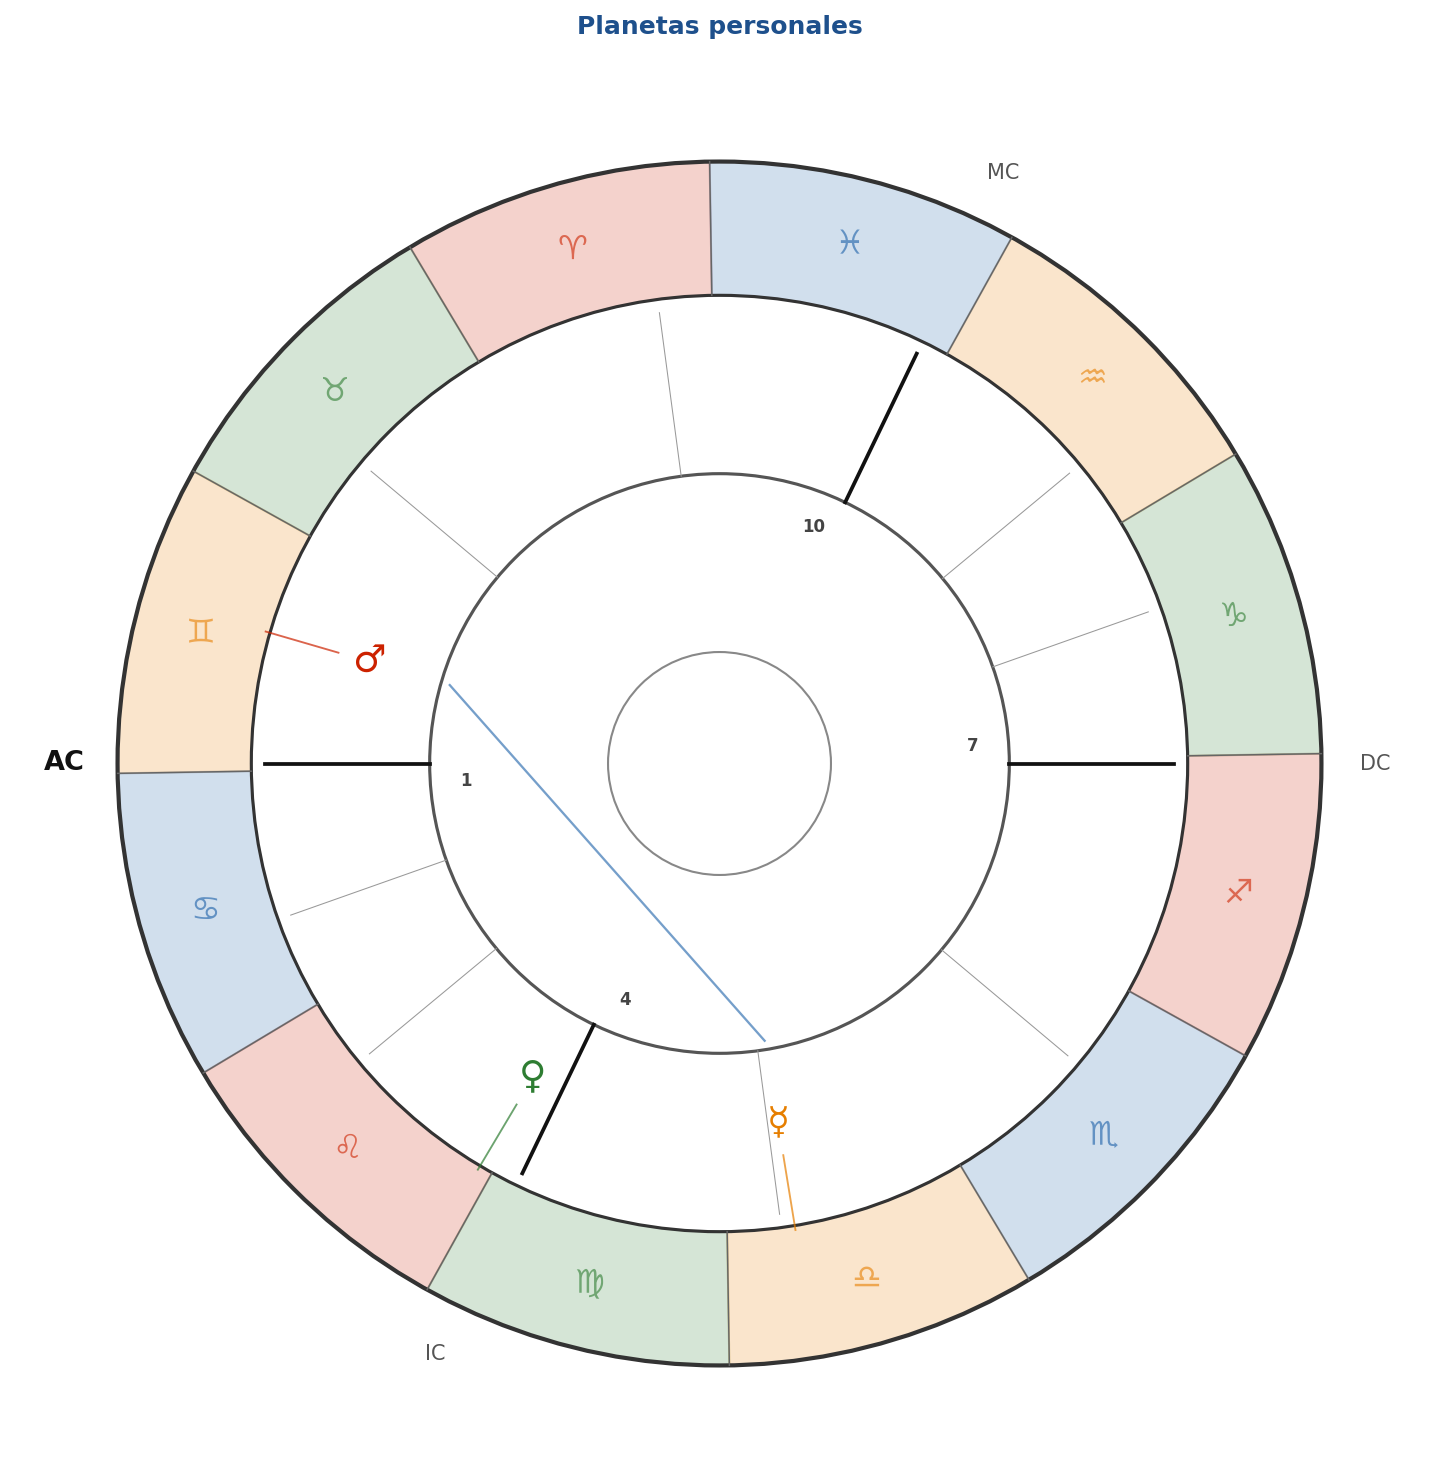
\includegraphics[width=0.72\textwidth]{Virginia_Riezu_Planetas_Personales_rueda.png}
\end{center}

\vspace{0.3cm}
\Needspace{5\baselineskip}

% ── Interpretación ────────────────────────────────────────────────────────────
\section{Interpretación — Arquitectura Interna}

\begin{center}
{\small\itshape\color{grisai}
No se trata de describir la personalidad.\\
Se trata de observar cómo procesas, cómo te vinculas\\
y cómo se mueve tu energía en la vida cotidiana.
}
\end{center}

\justifying

\vspace{0.8cm}

% ── 1. Funcionamiento general ─────────────────────────────────────────────────
\subsection{1. Funcionamiento general}

\justifying
Mercurio está en Libra, Casa 5: muestra cómo piensas, cómo ordenas lo que percibes y cómo traduces lo que ocurre en palabras o ideas.
Venus está en Leo, Casa 3: muestra cómo te vinculas, qué necesitas para sentir conexión y cómo buscas equilibrio afectivo.
Marte está en Géminis, Casa 12: muestra cómo se activa tu acción, cómo descargas energía y cómo respondes ante el impulso.

Hay coherencia elemental entre: tu forma de pensar (Mercurio) y tu forma de vincularte (Venus) se apoyan por elementos compatibles: Aire/Fuego; tu forma de pensar (Mercurio) y tu forma de actuar (Marte) comparten elemento: Aire; tu forma de vincularte (Venus) y tu forma de actuar (Marte) se apoyan por elementos compatibles: Fuego/Aire. Esto facilita que esas áreas colaboren entre sí. Aun así, lo que fluye con facilidad también puede volverse automático si no lo observas con consciencia.

Otros aspectos entre planetas personales: Mercurio–Marte en trígono (orbe 4.54°).

\vspace{0.8cm}

% ── 2. Mercurio ───────────────────────────────────────────────────────────────
\subsection{2. Mercurio — Pensamiento y procesamiento}

\subsubsection*{Mercurio en Libra — Casa 5}

\justifying
Tu mente funciona comparando perspectivas. Tiendes a ver automáticamente varios puntos de vista y buscas equilibrio antes de decidir. Esto aporta matices, capacidad de diálogo y sensibilidad relacional.

La saturación aparece cuando tienes que tomar una decisión sin haber encontrado suficiente equilibrio interno. Entonces sigues generando nuevas posibilidades incluso cuando ya hay información suficiente. El bloqueo suele aparecer especialmente en decisiones con carga relacional o emocional: si algo puede afectar a otras personas, tu mente permanece abierta más tiempo.

Sueles regularte mejor cuando puedes ordenar opciones por escrito, pensar en voz alta o poner límites temporales a las decisiones.

Necesitas creatividad, expresión y participación personal para activar la mente. Comprendes mejor cuando puedes jugar con las ideas, explicarlas a tu manera o transformarlas en algo creativo y vivo.

La saturación aparece cuando el pensamiento se vuelve excesivamente rígido, repetitivo o limitado a tareas puramente técnicas. Entonces disminuye el interés y la atención pierde vitalidad. Sueles regularte mejor cuando puedes crear, enseñar, explicar o expresarte de forma más libre.

En relación con los otros planetas personales:

Mercurio en trígono a Marte: pensamiento y acción colaboran de forma natural. Sueles organizar, decidir y ejecutar sin demasiada fricción interna.

La facilidad aporta rapidez y capacidad resolutiva, aunque a veces puede hacer que actúes tan fluidamente que no detectes momentos donde sería útil detenerte un poco más.

Sueles regularte bien mediante acción clara y objetivos concretos.

\vspace{0.8cm}

% ── 3. Venus ──────────────────────────────────────────────────────────────────
\subsection{3. Venus — Vínculo y regulación relacional}

\subsubsection*{Venus en Leo — Casa 3 (Rx)}

\justifying
Necesitas sentir reconocimiento genuino y apreciación real dentro del vínculo. La conexión suele fortalecerse cuando puedes mostrarte tal como eres y sentir que la otra persona realmente te ve.

La saturación aparece cuando la relación se vuelve únicamente funcional y desaparece la sensación de reconocimiento mutuo. Entonces puedes empezar a esforzarte más para recuperar atención o validación, y ese esfuerzo termina agotando. Cuando el vínculo deja de sostenerse, puedes volverte más distante, más teatral emocionalmente o retirarte por completo.

Sueles regularte mejor mediante calidez, reconocimiento sincero y relaciones donde puedes expresarte sin sentirte reducíde a una función.

Necesitas comunicación frecuente y movimiento relacional constante para sentir conexión. El vínculo suele nutrirse mediante conversación, intercambio cotidiano, humor y cercanía mental.

La saturación aparece cuando la relación pierde intercambio real o queda reducida únicamente a funciones prácticas o emociones densas. Entonces la conexión empieza a sentirse más distante aunque el vínculo continúe. Sueles regularte mejor mediante comunicación ligera, contacto frecuente y curiosidad mutua.

Venus está retrógrada. Tu forma de vincularte puede ser más interna, más reflexiva o necesitar revisión consciente. Puedes tardar más en reconocer qué necesitas en relación, qué contacto te resulta suficiente y qué tipo de vínculo puedes sostener.

\vspace{0.8cm}

% ── 4. Marte ──────────────────────────────────────────────────────────────────
\subsection{4. Marte — Acción y descarga}

\subsubsection*{Marte en Géminis — Casa 12}

\justifying
Tu energía se activa a través del pensamiento, la curiosidad y el intercambio mental. Necesitas movimiento cognitivo, variedad y estímulo para mantenerte en marcha. La acción descarga hablando, escribiendo, aprendiendo o cambiando de enfoque.

La saturación aparece cuando hay demasiados estímulos o demasiadas tareas abiertas al mismo tiempo. Entonces la energía se dispersa y cuesta terminar lo que empiezas. También puede aparecer inquietud verbal, aceleración mental o necesidad de discutir como forma de descarga.

Sueles regularte mejor mediante movimiento, conversación, escritura y actividades que permitan cambiar de foco sin perder dirección.

Tu energía tiende a funcionar hacia adentro y no siempre encuentra salida visible inmediata. Puedes acumular activación silenciosamente si no existen espacios seguros de descarga.

La saturación aparece cuando toda la energía queda retenida internamente o te adaptas constantemente a lo que otras personas necesitan sin registrar tu propio impulso. Entonces aparece agotamiento, confusión o sensación de pérdida de dirección. Sueles regularte mejor mediante descanso profundo, creatividad, práctica interior y actividades donde puedas actuar sin exceso de exposición externa.

\vspace{0.8cm}

% ── 5. Integración ────────────────────────────────────────────────────────────
\subsection{5. Integración — Coherencias, fricciones y bucles}

\justifying
Mercurio en trígono a Marte: pensamiento y acción colaboran de forma natural. Sueles organizar, decidir y ejecutar sin demasiada fricción interna.

La facilidad aporta rapidez y capacidad resolutiva, aunque a veces puede hacer que actúes tan fluidamente que no detectes momentos donde sería útil detenerte un poco más.

Sueles regularte bien mediante acción clara y objetivos concretos.

Cuando hay demasiada presión, puede aparecer una cadena reconocible: Mercurio en Libra multiplica perspectivas sin llegar a una dirección clara. Desde ahí, Venus en Leo se aleja del vínculo o usa la relación como escenario de descarga. Y Marte en Géminis genera agitación que no siempre produce movimiento real. El ciclo se cierra cuando la energía acumulada vuelve a saturar el punto inicial.

\vspace{0.8cm}

% ── 6. Orientación práctica ───────────────────────────────────────────────────
\subsection{6. Orientación práctica}

\subsubsection*{Desde dónde empezar}

\justifying
Desde tu forma de vincularte (Venus) en Leo, Casa 3. De las tres áreas, esta suele requerir menos energía para activarse. La entrada es activar el movimiento antes de intentar resolverlo todo mentalmente. Empezar por aquí puede abrir movimiento en el resto.

\subsubsection*{Qué sostener}

\justifying
Conviene sostener especialmente tu forma de pensar (Mercurio) en Libra: espacio mental, palabra clara e intercambio regulado. Bajo presión, esta área puede desorganizarse antes que las demás. Cuando se estabiliza, el resto de tu funcionamiento tiene más capacidad para reorganizarse.

\subsubsection*{Qué evitar}

\justifying
Evitar asumir que la ausencia de fricción visible significa que todo está bien. A veces los bucles no hacen ruido porque te has acostumbrado a funcionar así.

\vspace{0.6cm}

\justifying
Si no se sostiene: pensamiento, vínculo y acción empiezan a funcionar por separado. Lo que piensas no alimenta la acción, la acción no informa al vínculo y el vínculo no regula la energía disponible. El esfuerzo aumenta, la claridad disminuye y la saturación llega antes.

\vspace{1.2cm}

\begin{center}
{\small\itshape\color{grisai}
La astrología se utiliza aquí como lenguaje simbólico de observación,\\
no como una definición cerrada de quién eres.\\[0.2cm]
Este documento propone una lectura funcional y orientativa, no un diagnóstico.
}
\end{center}

\end{document}
